% =====================================================================
% Big Data — Final Project Report (Team 32)
% Title: Temporal Analysis and Prediction of Job Demand Using LinkedIn Data
%
% Compile with:
%   cd docs
%   pdflatex final_report.tex
%   pdflatex final_report.tex   % run twice for ToC + cross-references
%
% External figures (replace placeholders with your own PNGs/PDFs in
% docs/figures/ before final submission):
%   figures/architecture.pdf
%   figures/er_diagram.pdf
%   figures/eda_*.png             (EDA charts exported from Superset)
%   figures/dashboard_*.png       (dashboard screenshots)
%   figures/confusion_<model>.png (optional confusion-matrix plots)
%   figures/feature_importance.png
% =====================================================================
\documentclass[11pt,a4paper]{article}

\usepackage[utf8]{inputenc}
\usepackage[T1]{fontenc}
\usepackage{lmodern}
\usepackage[english]{babel}
\usepackage[a4paper,margin=1in]{geometry}
\usepackage{microtype}
\usepackage{graphicx}
\usepackage{xcolor}
\usepackage{booktabs}
\usepackage{longtable}
\usepackage{array}
\usepackage{tabularx}
\usepackage{multirow}
\usepackage{caption}
\usepackage{subcaption}
\usepackage{enumitem}
\usepackage{fancyhdr}
\usepackage{listings}
\usepackage{tikz}
\usetikzlibrary{shapes.geometric,arrows.meta,positioning,fit,calc}
\usepackage{hyperref}
\hypersetup{
  colorlinks=true,
  linkcolor=blue!50!black,
  urlcolor=blue!50!black,
  citecolor=blue!50!black,
  pdftitle={Big Data Final Project — LinkedIn Job Demand},
  pdfauthor={Team 32}
}

% -- Page style --
\pagestyle{fancy}
\fancyhf{}
\fancyhead[L]{\small Big Data Final Project --- Team 32}
\fancyhead[R]{\small\thepage}
\renewcommand{\headrulewidth}{0.4pt}

% -- Listing styles --
\definecolor{codegray}{rgb}{0.5,0.5,0.5}
\definecolor{codebg}{rgb}{0.97,0.97,0.97}
\definecolor{codekw}{rgb}{0.10,0.10,0.55}
\definecolor{codestr}{rgb}{0.50,0.10,0.10}
\definecolor{codecom}{rgb}{0.20,0.50,0.20}

\lstdefinestyle{plain}{
  backgroundcolor=\color{codebg},
  basicstyle=\ttfamily\footnotesize,
  commentstyle=\color{codecom}\itshape,
  keywordstyle=\color{codekw}\bfseries,
  stringstyle=\color{codestr},
  numbers=left,
  numberstyle=\tiny\color{codegray},
  numbersep=8pt,
  frame=single,
  rulecolor=\color{codegray!40},
  breaklines=true,
  breakatwhitespace=true,
  showstringspaces=false,
  captionpos=b,
  xleftmargin=12pt,
  framexleftmargin=8pt
}
\lstdefinestyle{python}{style=plain,language=Python}
\lstdefinestyle{sql}{style=plain,language=SQL,morekeywords={STRING,DOUBLE,BIGINT,PARQUET,STORED,LOCATION,EXTERNAL}}
\lstdefinestyle{bash}{style=plain,language=bash}

% -- Title block --
\title{
  \vspace{-1cm}
  \rule{\linewidth}{0.4pt}\\[6pt]
  {\Huge\bfseries Temporal Analysis and Prediction\\of Job Demand Using LinkedIn Data}\\[8pt]
  \rule{\linewidth}{0.4pt}\\
  \large Big Data --- Final Project Report
}
\author{
  Team 32 \\[2pt]
  \small
  Member 1 \quad Member 2 \quad Member 3 \quad Member 4 \\[6pt]
  Innopolis University
}
\date{2026}

\begin{document}

% =====================================================================
\begin{titlepage}
\centering
\vspace*{1cm}

{\scshape\Large Innopolis University \par}
\vspace{0.3cm}
{\scshape\large Big Data --- Final Project \par}

\vspace{2.5cm}
\rule{\linewidth}{0.6pt}\\[12pt]
{\Huge\bfseries Temporal Analysis and Prediction\\[4pt]of Job Demand Using LinkedIn Data\par}
\vspace{12pt}
\rule{\linewidth}{0.6pt}

\vspace{2cm}
{\Large Team 32\par}
\vspace{0.6cm}

\begin{tabular}{c}
\textbf{Emil Goryachih} --- Data Engineering (Stages 1, 2)\\[4pt]
\textbf{Vladislav Galkin} --- EDA \& Analytics (Stage 2)\\[4pt]
\textbf{Rodion Krainov} --- Machine Learning (Stage 3)\\[4pt]
\textbf{Vladislav Galkin} --- Dashboard \& Visualisation (Stage 4)\\
\end{tabular}

\vfill

\begin{tabular}{rl}
\textbf{Dataset:} & 1.3 M LinkedIn Jobs and Skills (2024) \\
\textbf{Task type:} & Binary classification (high vs.\ low demand) \\
\textbf{Best model:} & Gradient Boosted Trees, AUC ROC $0.94$ \\
\textbf{Repository:} & \texttt{bigdata-team32-linkedin-job-demand} \\
\end{tabular}

\vspace{1.5cm}
{\large \today\par}
\end{titlepage}

% =====================================================================
\tableofcontents
\newpage

% =====================================================================
\section{Introduction}
\label{sec:introduction}

The labour market is one of the most volatile, geographically uneven,
and information-rich domains in the modern economy.  Online job
platforms such as LinkedIn aggregate millions of postings every week,
each of which is a small signal about which roles, skills, companies
and regions are growing or contracting.  Aggregated across the
platform, those signals describe \emph{job demand}: the structural
pattern of where, what, and at what seniority companies need to hire.

\paragraph{Business objective.}
This project builds an end-to-end big data pipeline that turns 1.35
million raw LinkedIn job postings into actionable demand intelligence.
The pipeline answers two complementary business questions:

\begin{enumerate}[label=(Q\arabic*),leftmargin=*]
  \item \textbf{Descriptive:} where is hiring concentrated by country,
    role, seniority, work arrangement, and company? Which skills are
    most demanded globally and per country?
  \item \textbf{Predictive:} given a (country, position) combination,
    can we predict whether it is a \emph{high-demand} segment for that
    role family?
\end{enumerate}

Both outputs feed an interactive Apache Superset dashboard so that
business stakeholders --- recruiters, HR analysts, course designers
and policy researchers --- can drill into the market signal without
running any Spark job themselves.

\paragraph{Why big data.}
The raw dataset (\textbf{1\,348\,454} rows, \textbf{6.19 GB}) is too
large to process in a notebook on a single machine: the join between
postings, skills and summaries by itself produces hundreds of
millions of intermediate rows, and the per-position quantile
computations used for the ML label require a global sort.  The
project therefore uses the standard university Hadoop / YARN cluster
with Sqoop, Hive, Spark and Superset.  All training runs on the
cluster and all heavy artefacts live on HDFS.

\paragraph{Document structure.}
Section~\ref{sec:data} describes the dataset.  Section~\ref{sec:arch}
gives the high-level architecture and stage I/O.
Section~\ref{sec:prep} covers data preparation in PostgreSQL and Hive
(ER diagram, ingestion, Parquet/enriched tables).
Section~\ref{sec:eda} reports the eight EDA insights.
Section~\ref{sec:ml} is the machine-learning section: feature
engineering, four models with cross-validated grid search, evaluation,
soft-voting ensemble and sample predictions.
Section~\ref{sec:dashboard} documents the Superset dashboard.
Section~\ref{sec:conclusion} concludes, and
Section~\ref{sec:reflections} contains challenges, recommendations and
the per-task contribution table.

% =====================================================================
\section{Data Description}
\label{sec:data}

\subsection{Source}
The dataset is the public Kaggle dataset
\textit{1.3M LinkedIn Jobs and Skills (2024)} by Aniczka
\cite{kaggle-linkedin-2024}.  It is composed of three CSV files joined
on the natural key \texttt{job\_link}:

\begin{center}
\begin{tabularx}{\linewidth}{l l r X}
\toprule
\textbf{File} & \textbf{Records} & \textbf{Size} & \textbf{Role} \\
\midrule
\texttt{linkedin\_job\_postings.csv} & 1\,348\,454 & $\approx$ 380 MB & Posting metadata, location, level, type \\
\texttt{job\_skills.csv}             & 1\,296\,381 & $\approx$ 850 MB & Comma-separated skill list per posting \\
\texttt{job\_summary.csv}            & 1\,297\,332 & $\approx$ 5.0 GB & Long-form job description text \\
\midrule
\textbf{Total}                       & --- & \textbf{$\approx$ 6.19 GB} & --- \\
\bottomrule
\end{tabularx}
\end{center}

\subsection{Feature description}
After joining the three files on \texttt{job\_link}, every row is one
LinkedIn job posting with the columns listed in Table~\ref{tab:cols}.

\begin{table}[h]
\centering
\caption{Columns of the joined LinkedIn job-postings table.}
\label{tab:cols}
\small
\begin{tabularx}{\linewidth}{l l X}
\toprule
\textbf{Column} & \textbf{Type} & \textbf{Description} \\
\midrule
\texttt{job\_link}            & STRING     & Unique LinkedIn job URL (primary key). \\
\texttt{last\_processed\_time}& TIMESTAMPTZ& Timestamp the scraper last updated the record. \\
\texttt{got\_summary}         & BOOLEAN    & Whether a job summary was scraped. \\
\texttt{got\_ner}             & BOOLEAN    & Whether named-entity recognition ran on the summary. \\
\texttt{is\_being\_worked}    & BOOLEAN    & Scraper internal flag. \\
\texttt{job\_title}           & STRING     & Free-text title written by the recruiter. \\
\texttt{company}              & STRING     & Hiring company. \\
\texttt{job\_location}        & STRING     & Free-text location string. \\
\texttt{first\_seen}          & DATE       & Date the scraper first observed the posting. \\
\texttt{search\_city}         & STRING     & City used in the search that returned this posting. \\
\texttt{search\_country}      & STRING     & Country used in the search. \\
\texttt{search\_position}     & STRING     & Normalised role keyword used in the search. \\
\texttt{job\_level}           & STRING     & Seniority label (Entry, Associate, Mid--Senior, Director, Internship). \\
\texttt{job\_type}            & STRING     & Work arrangement (Onsite, Remote, Hybrid, Full-time, Part-time, Contract). \\
\texttt{job\_skills}          & STRING     & Comma-separated list of required skills. \\
\texttt{job\_summary}         & STRING     & Long-form job description. \\
\bottomrule
\end{tabularx}
\end{table}

\subsection{Dataset criteria compliance}
The course rubric \cite{bs-final-project} requires
\textbf{$\geq 500$\,k records}, \textbf{$\geq 500$ MB}, \textbf{$\geq
6$ explanatory features}, and either a \emph{datetime} or a
\emph{geospatial} feature (date-only does not count).  Our dataset
satisfies all four:

\begin{itemize}[leftmargin=*]
  \item \textbf{Records:} 1\,348\,454 $\gg$ 500\,000.
  \item \textbf{Size:} 6.19 GB $\gg$ 500 MB.
  \item \textbf{Features:} 13 raw explanatory columns (10 after
    dropping scraper-internal flags), well above the 6-column
    minimum.
  \item \textbf{Datetime:} \texttt{last\_processed\_time} is a
    \texttt{TIMESTAMPTZ} (date + time + zone).
  \item \textbf{Geospatial:} \texttt{search\_country},
    \texttt{search\_city} and the free-text \texttt{job\_location}
    give country/city granularity for every posting.
\end{itemize}

\subsection{Coverage and quality}
After loading into Hive Parquet, row counts of each source layer are
shown in Table~\ref{tab:counts}.  Coverage of the optional auxiliary
files is very high: 96.0\% of postings have an associated skill list
and 96.2\% have a summary.

\begin{table}[h]
\centering
\caption{Row counts and join coverage at the enriched layer.}
\label{tab:counts}
\small
\begin{tabular}{lrr}
\toprule
\textbf{Table} & \textbf{Rows} & \textbf{\% of postings} \\
\midrule
\texttt{linkedin\_job\_postings\_parquet}  & 1\,348\,454 & 100.0\% \\
\texttt{job\_skills\_parquet}              & 1\,296\,381 & 96.1\%  \\
\texttt{job\_summary\_parquet}             & 1\,297\,332 & 96.2\%  \\
\texttt{linkedin\_jobs\_enriched} (LEFT JOIN) & 1\,348\,454 & 100.0\% \\
\quad of which have skills                    & 1\,294\,374 & 96.0\% \\
\quad of which have summary                   & 1\,297\,332 & 96.2\% \\
\bottomrule
\end{tabular}
\end{table}

% =====================================================================
\section{Architecture of the Data Pipeline}
\label{sec:arch}

The pipeline is split into four stages plus a preprocessing and a
postprocessing step, orchestrated by the top-level
\texttt{main.sh}.  Figure~\ref{fig:arch} shows the end-to-end data
flow.

\begin{figure}[h]
\centering
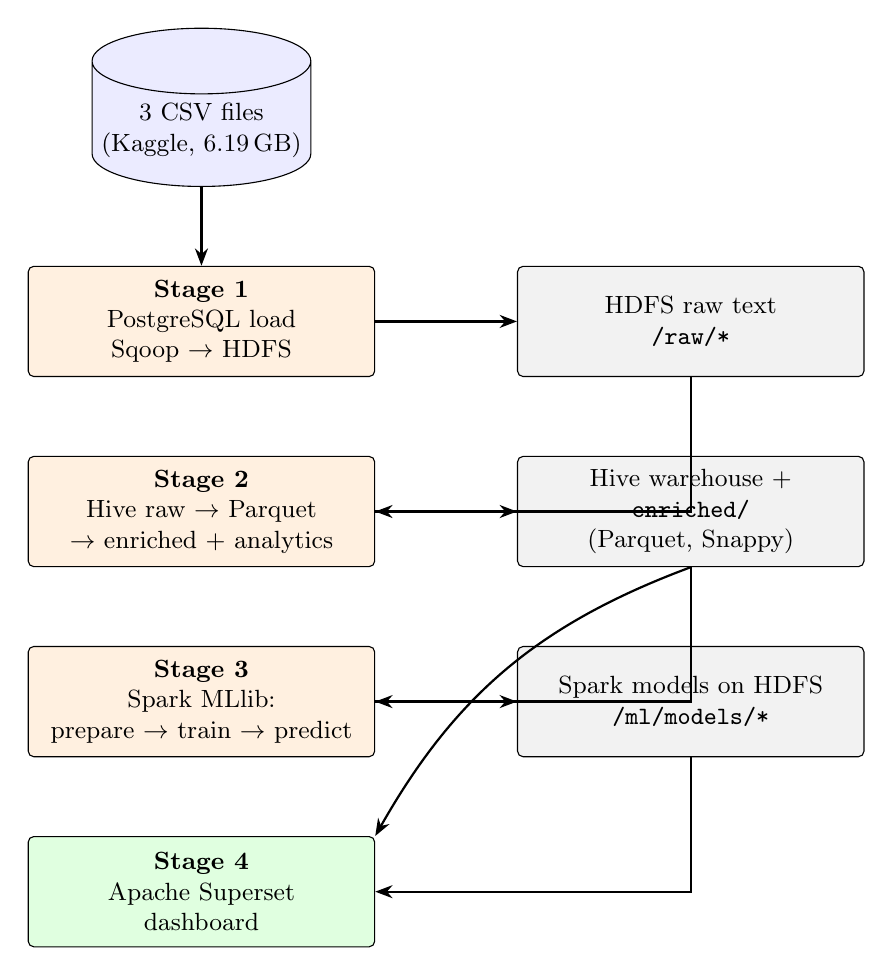
\begin{tikzpicture}[
  node distance=10mm and 18mm,
  every node/.style={font=\small},
  source/.style={cylinder, shape border rotate=90, aspect=0.3, draw,
                 fill=blue!8, minimum height=14mm, minimum width=24mm,
                 align=center},
  stage/.style ={rectangle, draw, rounded corners=2pt, fill=orange!12,
                 minimum height=14mm, minimum width=44mm, align=center},
  sink/.style  ={rectangle, draw, rounded corners=2pt, fill=green!12,
                 minimum height=14mm, minimum width=44mm, align=center},
  arr/.style   ={-{Stealth[length=2.2mm]}, thick}
]
  \node[source]                       (csv)   {3 CSV files\\(Kaggle, 6.19\,GB)};
  \node[stage,  below=of csv]         (s1)    {\textbf{Stage 1}\\PostgreSQL load\\Sqoop $\rightarrow$ HDFS};
  \node[stage,  below=of s1]          (s2)    {\textbf{Stage 2}\\Hive raw $\rightarrow$ Parquet\\$\rightarrow$ enriched + analytics};
  \node[stage,  below=of s2]          (s3)    {\textbf{Stage 3}\\Spark MLlib:\\prepare $\rightarrow$ train $\rightarrow$ predict};
  \node[sink,   below=of s3]          (s4)    {\textbf{Stage 4}\\Apache Superset\\dashboard};

  \node[stage, right=of s1, fill=gray!10] (hdfs1) {HDFS raw text\\\texttt{/raw/*}};
  \node[stage, right=of s2, fill=gray!10] (hdfs2) {Hive warehouse +\\\texttt{enriched/}\\(Parquet, Snappy)};
  \node[stage, right=of s3, fill=gray!10] (hdfs3) {Spark models on HDFS\\\texttt{/ml/models/*}};

  \draw[arr] (csv)   -- (s1);
  \draw[arr] (s1)    -- (hdfs1);
  \draw[arr] (hdfs1) |- (s2);
  \draw[arr] (s2)    -- (hdfs2);
  \draw[arr] (hdfs2) |- (s3);
  \draw[arr] (s3)    -- (hdfs3);
  \draw[arr] (hdfs3) |- (s4);
  \draw[arr] (hdfs2.south) to[bend right=20] (s4.north east);
\end{tikzpicture}
\caption{End-to-end pipeline.  All heavy artefacts live on HDFS;
local \texttt{output/} only holds small summary files for the
grader.}
\label{fig:arch}
\end{figure}

\subsection{Per-stage input / output}
Table~\ref{tab:stages} summarises what each stage consumes and
produces.

\begin{table}[h]
\centering
\caption{Per-stage input/output contract.}
\label{tab:stages}
\small
\begin{tabularx}{\linewidth}{l X X}
\toprule
\textbf{Stage} & \textbf{Input} & \textbf{Output} \\
\midrule
1 (Ingestion) & 3 local CSV files & PostgreSQL tables; HDFS raw text under \texttt{/user/team32/linkedin/raw/} \\
2 (Storage)   & HDFS raw text     & Hive Parquet tables (raw, parquet, enriched, $\sim$14 analytics tables) \\
3 (ML)        & \texttt{linkedin\_jobs\_enriched} Parquet & 4 saved \texttt{PipelineModel}s on HDFS, metrics + CV grids + confusion + feature importance under local \texttt{output/} \\
4 (Dashboard) & Hive analytics tables + ML metrics & Apache Superset dashboard + dashboard planning artefacts in \texttt{output/} \\
\bottomrule
\end{tabularx}
\end{table}

\subsection{Technology stack}
\begin{center}
\small
\begin{tabular}{l l}
\toprule
\textbf{Layer} & \textbf{Tool / Version} \\
\midrule
Relational store   & PostgreSQL 16 \\
Ingest to HDFS     & Apache Sqoop (MapReduce engine) \\
File system        & HDFS \\
Warehouse          & Apache Hive (Parquet, Snappy, Tez) \\
Compute            & Apache Spark 3.x (Spark SQL, MLlib) \\
Resource manager   & Hadoop YARN \\
Dashboard          & Apache Superset \\
Code quality       & pylint \\
Cluster Python     & 3.6 (constrains language features) \\
\bottomrule
\end{tabular}
\end{center}

% =====================================================================
\section{Data Preparation}
\label{sec:prep}

\subsection{PostgreSQL relational model}
The Stage 1 schema (\texttt{sql/postgres/01\_create\_tables.sql})
mirrors the three CSV files and enforces referential integrity by
using \texttt{job\_link} as the primary key of the postings table and
adding two indexed many-to-one tables for skills and summaries.
Figure~\ref{fig:er} is the entity-relationship diagram.

\begin{figure}[h]
\centering
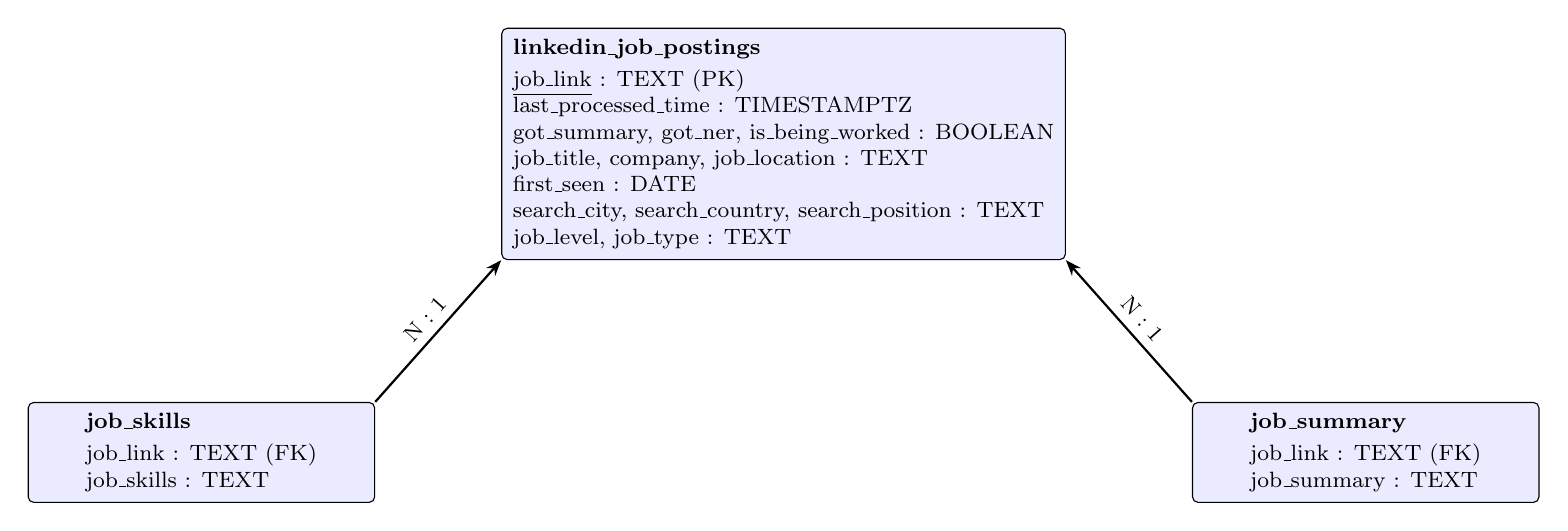
\begin{tikzpicture}[
  node distance=18mm and 10mm,
  every node/.style={font=\footnotesize},
  entity/.style ={rectangle, draw, fill=blue!8, rounded corners=2pt,
                  minimum width=44mm, align=left, inner sep=4pt},
  rel/.style    ={-{Stealth[length=2mm]}, thick}
]
\node[entity] (jp) {
  \textbf{linkedin\_job\_postings}\\[2pt]
  \underline{job\_link} : TEXT (PK)\\
  last\_processed\_time : TIMESTAMPTZ\\
  got\_summary, got\_ner, is\_being\_worked : BOOLEAN\\
  job\_title, company, job\_location : TEXT\\
  first\_seen : DATE\\
  search\_city, search\_country, search\_position : TEXT\\
  job\_level, job\_type : TEXT
};
\node[entity, below left=of jp, xshift=-6mm] (sk) {
  \textbf{job\_skills}\\[2pt]
  job\_link : TEXT (FK)\\
  job\_skills : TEXT
};
\node[entity, below right=of jp, xshift=6mm] (sm) {
  \textbf{job\_summary}\\[2pt]
  job\_link : TEXT (FK)\\
  job\_summary : TEXT
};
\draw[rel] (sk.north east) -- node[above,sloped]{N : 1} (jp.south west);
\draw[rel] (sm.north west) -- node[above,sloped]{N : 1} (jp.south east);
\end{tikzpicture}
\caption{PostgreSQL entity-relationship diagram. \texttt{job\_link}
links the three tables; indexes on this column accelerate the
downstream Sqoop import.}
\label{fig:er}
\end{figure}

The postings table is the parent; the skills and summary tables are
many-to-one children (a given posting can have multiple comma-merged
skill rows in raw data, hence \texttt{N:1} is a safe upper bound).
Indexes accelerate Sqoop's split-by query and Hive joins.

\subsection{Loading and quality checks}
\texttt{scripts/load\_postgres.py} streams each CSV via
\texttt{psycopg2}'s \texttt{COPY} into the corresponding PostgreSQL
table and then runs \texttt{sql/postgres/03\_quality\_checks.sql} to
report:

\begin{itemize}[leftmargin=*]
  \item Row counts and distinct \texttt{job\_link} values per table.
  \item Min/max of \texttt{first\_seen} and \texttt{last\_processed\_time}.
  \item Join coverage between postings and the two auxiliary tables.
  \item Distribution of \texttt{job\_level} and \texttt{job\_type}.
\end{itemize}

Results are written to
\texttt{output/stage1\_postgres\_quality\_checks.txt}.

\subsection{Sqoop import to HDFS}
\texttt{scripts/stage1\_sqoop\_import.sh} imports each PostgreSQL
table to HDFS as text files using Hadoop MapReduce.  Listing
\ref{lst:sqoop} shows the canonical invocation.

\begin{lstlisting}[style=bash,caption={Sqoop import of one of the
three PostgreSQL tables.},label={lst:sqoop}]
sqoop import \
  --connect "$JDBC_URL" \
  --username "$DB_USER" \
  --password "$DB_PASSWORD" \
  --table linkedin_job_postings \
  --target-dir "$HDFS_BASE/raw/linkedin_job_postings" \
  --as-textfile \
  --fields-terminated-by '\001' \
  --lines-terminated-by '\n' \
  --null-string '\\N' \
  --null-non-string '\\N' \
  --hive-drop-import-delims
\end{lstlisting}

\subsection{Hive layers: raw $\rightarrow$ Parquet $\rightarrow$ enriched}
Stage 2 builds three Hive layers with progressive transformations:

\begin{enumerate}[leftmargin=*]
  \item \textbf{Raw external tables}
    (\texttt{01\_create\_raw\_tables.hql}) point at the Sqoop output
    with no copy; all columns are \texttt{STRING}.
  \item \textbf{Parquet tables}
    (\texttt{02\_create\_parquet\_tables.hql}) cast booleans and
    dates, drop carriage returns, normalise NULL strings, and
    re-store as Snappy-compressed Parquet for analytical workloads.
  \item \textbf{Enriched table}
    (\texttt{03\_create\_enriched\_table.hql}) is a left join of
    postings $\bowtie$ skills $\bowtie$ summary on \texttt{job\_link}
    and is the canonical source of truth for Stage 3 and the
    dashboard.
\end{enumerate}

Listing~\ref{lst:enriched} shows the enriched-table DDL.

\begin{lstlisting}[style=sql,caption={Enriched Hive table
construction.},label={lst:enriched}]
CREATE TABLE linkedin_jobs_enriched
STORED AS PARQUET
TBLPROPERTIES ('parquet.compression'='SNAPPY')
AS
SELECT
    p.job_link, p.first_seen, p.last_processed_time,
    p.job_title, p.company, p.job_location,
    p.search_city, p.search_country, p.search_position,
    p.job_level, p.job_type,
    s.job_skills, sm.job_summary,
    p.got_summary, p.got_ner, p.is_being_worked
FROM linkedin_job_postings_parquet p
LEFT JOIN job_skills_parquet   s  ON p.job_link = s.job_link
LEFT JOIN job_summary_parquet  sm ON p.job_link = sm.job_link;
\end{lstlisting}

A sample of the enriched table is shown in
Table~\ref{tab:enriched-sample}.

\begin{table}[h]
\centering
\caption{Three example rows from \texttt{linkedin\_jobs\_enriched}
(truncated; skill / summary columns abbreviated).}
\label{tab:enriched-sample}
\scriptsize
\begin{tabularx}{\linewidth}{l l l l l X}
\toprule
\textbf{job\_title} & \textbf{country} & \textbf{position} & \textbf{level} & \textbf{type} & \textbf{skills (first few)} \\
\midrule
Senior Software Engineer & United States   & software engineer & Mid--Senior & Full-time & Python, AWS, Docker, Kubernetes \\
Data Scientist           & United Kingdom  & data scientist    & Mid--Senior & Remote     & Python, SQL, Spark, ML \\
Product Manager          & Germany         & product manager   & Mid--Senior & Hybrid     & Agile, Roadmap, Stakeholders \\
\bottomrule
\end{tabularx}
\end{table}

\subsection{HDFS layout summary}
\begin{lstlisting}[style=plain,caption={HDFS directory layout after
Stage 2.}]
/user/team32/linkedin/
  raw/                          (Sqoop text files, Stage 1)
    linkedin_job_postings/
    job_skills/
    job_summary/
  warehouse/                    (Hive default DB warehouse)
  parquet/                      (Stage 2.2 Parquet copies)
    linkedin_job_postings_parquet/
    job_skills_parquet/
    job_summary_parquet/
  enriched/
    linkedin_jobs_enriched/     (1.35 M rows, ~1.9 GB Parquet)
  analytics/                    (Hive EDA tables, Stage 2.3)
    analytics_top_positions_global/
    analytics_top_skills_global/
    ...
  ml/                           (Stage 3 outputs)
    dataset_train/
    dataset_test/
    models/{rf,gbt,svm,nb}/
\end{lstlisting}

Total HDFS usage after Stages 1--3 is approximately 15 GB replicated
(5 GB logical), well under the 32 GB team quota.

% =====================================================================
\section{Data Analysis (EDA)}
\label{sec:eda}

The EDA layer is implemented in two parallel ways, both reading the
same enriched Parquet table:

\begin{enumerate}[leftmargin=*]
  \item HiveQL on Tez engine
    (\texttt{sql/hive/05\_analytics\_queries.hql}) materialises
    Snappy-compressed Parquet \texttt{analytics\_*} tables under
    \texttt{/user/team32/linkedin/analytics/}, which Superset connects
    to directly.
  \item Spark SQL on YARN
    (\texttt{scripts/stage2\_spark\_eda.py}) reads the same enriched
    Parquet and writes parallel analytics under
    \texttt{/analytics\_spark/} plus small CSV previews in
    \texttt{output/}.
\end{enumerate}

This dual implementation lets the team compare Hive and Spark
execution plans on the same questions and gives the dashboard a
redundant data source.  Below we list the eight business insights
produced; each was visualised in Superset
(Section~\ref{sec:dashboard}) with its own chart and accompanying
narrative.

\subsection{Insight 1 --- Global role demand}
\textbf{Source:} \texttt{analytics\_top\_positions\_global}.\\
\textbf{Query summary:} count of postings grouped by
\texttt{search\_position}, sorted descending.\\
\textbf{Chart:} horizontal bar chart, \texttt{search\_position} on the
$y$-axis, \texttt{posting\_count} on the $x$-axis.\\
\textbf{Storytelling:} the chart identifies which job roles dominate
global LinkedIn demand.  ``Software engineer'', ``data scientist'' and
``product manager'' anchor the top of the distribution, with a long
tail of more specialised roles.  Stakeholders use this view to
prioritise hiring plans, curriculum design and talent-acquisition
budgets around the roles with the largest market signal.

\subsection{Insight 2 --- Country-specific role demand}
\textbf{Source:} \texttt{analytics\_top\_positions\_by\_country}
and \texttt{analytics\_country\_position\_matrix}.\\
\textbf{Chart:} heatmap, $x$ = \texttt{search\_position},
$y$ = \texttt{search\_country}, colour = \texttt{posting\_count}.\\
\textbf{Storytelling:} demand is not uniform geographically.  Some
roles are concentrated in a few markets (e.g.\ specialised quantitative
roles cluster in the United States and the United Kingdom) while
others are broadly distributed.  Companies use this view for
region-specific recruiting and expansion decisions.

\subsection{Insight 3 --- Global skill demand}
\textbf{Source:} \texttt{analytics\_top\_skills\_global}.\\
\textbf{Query summary:} explode the comma-separated
\texttt{job\_skills} column, lowercase and trim each skill, then count
mentions globally.\\
\textbf{Chart:} bar chart, \texttt{skill} on $y$, \texttt{skill\_mentions}
on $x$.\\
\textbf{Storytelling:} the top skills (Python, SQL, communication,
project management, Excel) are diagnostic of what employers expect
across the dataset.  Candidates use this to prioritise learning and
companies compare their job descriptions against market norms.

\subsection{Insight 4 --- Skill demand by country}
\textbf{Source:} \texttt{analytics\_top\_skills\_by\_country}.\\
\textbf{Chart:} filterable horizontal bar chart, with a Superset
filter on \texttt{search\_country}.\\
\textbf{Storytelling:} skill demand has strong local variation
because regional industries and technical stacks differ.  This view
supports localised hiring and training strategies instead of assuming
a single global skill profile.

\subsection{Insight 5 --- Skills by seniority level}
\textbf{Source:} \texttt{analytics\_skills\_by\_job\_level}.\\
\textbf{Chart:} stacked bar chart of (skill, level) mentions.\\
\textbf{Storytelling:} junior, mid-level, and senior roles ask for
different skills.  Entry roles emphasise foundations and tools;
mid--senior roles ask for ownership and architecture; director roles
emphasise people and strategy.  This explains career progression and
shows which capabilities become more important at higher seniority.

\subsection{Insight 6 --- Job type / work arrangement distribution}
\textbf{Source:} \texttt{analytics\_job\_type\_distribution}.\\
\textbf{Chart:} pie or bar chart, $x$ = \texttt{job\_type},
$y$ = \texttt{posting\_pct}.\\
\textbf{Storytelling:} the market is split into onsite, hybrid and
remote arrangements with a smaller share of contract and internship
positions.  Hiring teams use this to benchmark whether their offers
match market expectations and whether they over- or under-index on a
particular arrangement.

\subsection{Insight 7 --- Top hiring companies}
\textbf{Source:} \texttt{analytics\_top\_companies}.\\
\textbf{Chart:} bar chart, $x$ = \texttt{company},
$y$ = \texttt{posting\_count}.\\
\textbf{Storytelling:} the companies posting the most jobs are the
strongest demand drivers in the market.  They are simultaneously
talent competitors and market signals.  Recruiters monitor this list
for benchmarking and to identify whom they are competing with for
candidates.

\subsection{Insight 8 --- Demand over time}
\textbf{Source:} \texttt{analytics\_demand\_by\_date}.\\
\textbf{Chart:} time-series line chart, $x$ = \texttt{first\_seen},
$y$ = \texttt{posting\_count}.\\
\textbf{Storytelling:} the time-series view shows how the volume of
new postings changes across the collection window.  The dataset's
\texttt{first\_seen} values are clustered in a 6-day scrape window in
January 2024, which is itself an important business observation: any
``temporal'' analysis on this dataset is therefore really within-week
analysis, and the data should not be used to make claims about
seasonality without an additional scrape (see
Section~\ref{sec:reflections}).

% =====================================================================
\section{Machine Learning Modeling}
\label{sec:ml}

Stage 3 turns the descriptive EDA into a predictive task.  The full
pipeline is implemented in three PySpark scripts under
\texttt{scripts/} and orchestrated by \texttt{scripts/stage3.sh}; the
detailed methodology and per-model analysis are in
\texttt{docs/stage3\_ml\_report.md} which complements this section.

\subsection{Predictive task and label engineering}
\paragraph{Task.}  Binary classification: predict whether a
\texttt{(search\_country, search\_position)} group is in the
\emph{high demand} segment of its role family.

\paragraph{Label.}  The label is not present in the source data;
it is engineered in
\texttt{scripts/stage3\_prepare\_dataset.py}:

\begin{lstlisting}[style=python,caption={Label engineering: per-position
top-quartile threshold.}]
thresholds = (
    df.groupBy("search_position")
      .agg(F.expr("percentile_approx(group_count, 0.75)")
             .alias("cat_threshold"))
)
joined = df.join(F.broadcast(thresholds), "search_position")
joined.withColumn(
    "high_demand",
    F.when(F.col("group_count") > F.col("cat_threshold"), 1)
     .otherwise(0)
     .cast(IntegerType())
)
\end{lstlisting}

Choosing the threshold \emph{per position} (rather than globally)
prevents the model from trivially learning ``software engineer is
always high, ceramic artist is always low.''  Instead, the classifier
has to identify which countries are above the typical demand for the
role.  The resulting class balance is approximately 13.5\% positive
/ 86.5\% negative.

\paragraph{Why no temporal features.}  The original plan was a weekly
\texttt{(week, country, position)} aggregation with lag/rolling
features.  Empirically, however, \texttt{first\_seen} covers only the
6-day scrape window of January 12 -- 17, 2024: there are not enough
buckets per group to build meaningful lag signals (the median
\texttt{(country, position)} group has one or two distinct dates).
The pipeline was simplified to a static aggregation, and this report
is honest about that constraint.

\subsection{Feature engineering}
For every \texttt{(country, position)} group the prepare script emits:

\begin{table}[h]
\centering
\caption{Feature set for Stage 3.}
\label{tab:features}
\small
\begin{tabularx}{\linewidth}{l l X}
\toprule
\textbf{Feature} & \textbf{Type} & \textbf{Why it is leak-free} \\
\midrule
\texttt{summary\_coverage}     & numeric ratio & proportion in [0, 1], independent of \texttt{group\_count} \\
\texttt{skills\_per\_posting}  & numeric ratio & \texttt{distinct\_skills / group\_count} \\
\texttt{companies\_per\_posting}& numeric ratio& \texttt{distinct\_companies / group\_count} \\
\texttt{distinct\_job\_levels} & numeric (1..5)& bounded by 5; very weak correlation with the label \\
\texttt{distinct\_job\_types}  & numeric       & same idea \\
\texttt{search\_country}       & categorical   & one-hot via \texttt{StringIndexer + OneHotEncoder} \\
\texttt{search\_position}      & categorical   & one-hot, same pipeline \\
\bottomrule
\end{tabularx}
\end{table}

\paragraph{Why ratios, not counts?}
\texttt{group\_count} itself is excluded because the label is a
deterministic function of it.  Raw \texttt{distinct\_companies} and
\texttt{distinct\_skills} are also excluded because their upper bound
is \texttt{group\_count}: large groups can have more distinct values
just by sample size, so they leak the label.  The ratio variants are
not bounded by \texttt{group\_count} in the same way --- they
describe market \emph{concentration}, not market \emph{size}.

\paragraph{Encoding and scaling.}
Categoricals go through \texttt{StringIndexer($handleInvalid$=keep)}
followed by \texttt{OneHotEncoder} and are concatenated with the five
numeric ratios by a \texttt{VectorAssembler}, producing a sparse
vector of approximately 1\,662 dimensions.  Per-model scaling
choices:

\begin{itemize}[leftmargin=*]
  \item Random Forest, Gradient Boosted Trees: no scaling (tree
    ensembles are invariant to monotonic feature transforms).
  \item Linear SVC: \texttt{StandardScaler(withMean=False,
    withStd=True)}.  Skipping the mean-centring keeps the one-hot
    vectors sparse and non-negative.
  \item Gaussian Naive Bayes: no scaling.  Gaussian NB models each
    feature as a per-class normal distribution and does not require
    non-negative inputs (unlike multinomial NB).
\end{itemize}

\subsection{Train / test split}
The rubric requires a 70/30 split with at least 60\% training data.
We use \texttt{DataFrame.randomSplit([0.7, 0.3], seed=42)} on the
filtered group-level frame.  The test set is \textbf{never} touched
during hyperparameter tuning --- only on the final evaluation
(Section~\ref{sec:ml-results}).  After filtering groups with
\texttt{group\_count $<$ 5} the dataset contains 4\,426 groups, of
which 3\,098 are train and 1\,328 are test (approximately).

\subsection{Models and hyperparameter grids}
Four classifiers plus a soft-voting ensemble are trained:

\begin{itemize}[leftmargin=*]
  \item Random Forest --- \texttt{RandomForestClassifier}
  \item Gradient Boosted Trees --- \texttt{GBTClassifier} (extra
    model beyond the rubric requirement)
  \item Linear Support Vector Machine --- \texttt{LinearSVC}
  \item Naive Bayes (Gaussian / Multinomial / Complement, chosen by
    CV) --- \texttt{NaiveBayes}
  \item Soft-voting ensemble of RF + GBT + SVM --- bonus
\end{itemize}

For every model we build a \textbf{$3 \times 3 \times 3 = 27$}
hyperparameter grid (one algorithm-level parameter plus two
model-level parameters, with \texttt{maxIter} explicitly excluded
because the rubric forbids iteration counts as hyperparameters).
Table~\ref{tab:grids} summarises the grids.

\begin{table}[h]
\centering
\caption{Hyperparameter grids.  ``A'' = algorithm hyperparameter,
``M'' = model hyperparameter.}
\label{tab:grids}
\small
\begin{tabularx}{\linewidth}{l X X X}
\toprule
\textbf{Model} & \textbf{Param 1 (A)} & \textbf{Param 2 (M)} & \textbf{Param 3 (M)} \\
\midrule
RF  & \texttt{numTrees} $\in$ \{50, 100, 200\}            & \texttt{maxDepth} $\in$ \{5, 10, 15\}      & \texttt{minInstancesPerNode} $\in$ \{1, 5, 10\} \\
GBT & \texttt{stepSize} $\in$ \{0.05, 0.1, 0.2\}           & \texttt{maxDepth} $\in$ \{3, 5, 8\}        & \texttt{minInstancesPerNode} $\in$ \{1, 5, 10\} \\
SVM & \texttt{aggregationDepth} $\in$ \{2, 3, 4\}          & \texttt{regParam} $\in$ \{0.01, 0.1, 1.0\} & \texttt{threshold} $\in$ \{-0.2, 0.0, 0.2\} \\
NB  & \texttt{modelType} $\in$ \{gaussian, multinomial, complement\} & \texttt{smoothing} $\in$ \{0.1, 1.0, 5.0\} & \texttt{thresholds} $\in$ \{[0.3,0.7], [0.5,0.5], [0.7,0.3]\} \\
\bottomrule
\end{tabularx}
\end{table}

\subsection{Cross-validation protocol}
Every model is wrapped in a Spark
\texttt{CrossValidator} with $k = 3$ folds, a
\texttt{MulticlassClassificationEvaluator(metricName=}\textit{f1}\texttt{)},
\texttt{parallelism=2} and the seed fixed at 42:

\begin{lstlisting}[style=python,caption={Cross-validated grid search
for one model.}]
cv = CrossValidator(
    estimator=pipeline,
    estimatorParamMaps=grid,        # 27 combinations
    evaluator=MulticlassClassificationEvaluator(
        labelCol="high_demand",
        predictionCol="prediction",
        metricName="f1"),
    numFolds=3,
    parallelism=2,
    seed=42)
cv_model = cv.fit(train)
predictions = cv_model.transform(test)
\end{lstlisting}

For every model we therefore run $27 \times 3 + 1 = 82$ fits (the
final \texttt{+1} is the refit of the winning combination on the full
training set).  Across all four models this is $\approx$ 328 fits per
pipeline run.  The full grid scores are saved to
\texttt{output/stage3\_<model>\_cv\_grid.csv}, sorted descending by
mean validation F1, so the tuning process is fully auditable.

\subsection{Evaluation metrics}
Because the task is \emph{binary} classification, we report the two
metrics the rubric requires for binary tasks plus accuracy and
weighted F1 for completeness:

\begin{itemize}[leftmargin=*]
  \item \textbf{Accuracy} --- fraction of correct predictions.
  \item \textbf{F1 (weighted)} --- harmonic mean of precision and
    recall, weighted by class frequency.
  \item \textbf{AUC ROC} --- area under the receiver-operating
    characteristic curve.  Probability that a random positive scores
    higher than a random negative.
  \item \textbf{AUC PR} --- area under the precision/recall curve.
    More informative than AUC ROC on a 13/87 class imbalance
    (random baseline = 0.135).
\end{itemize}

\subsection{Results}
\label{sec:ml-results}

\begin{table}[h]
\centering
\caption{Test-set metrics. GBT dominates accuracy, F1, and both AUCs.}
\label{tab:metrics}
\small
\begin{tabular}{lrrrr}
\toprule
\textbf{Model} & \textbf{Accuracy} & \textbf{F1} & \textbf{AUC ROC} & \textbf{AUC PR} \\
\midrule
\textbf{Gradient Boosted Trees} & \textbf{0.906} & \textbf{0.902} & \textbf{0.941} & \textbf{0.703} \\
Soft-voting ensemble (RF + GBT + SVM) & 0.891 & 0.875 & 0.931 & --- \\
Random Forest & 0.868 & 0.806 & 0.908 & 0.447 \\
Linear SVC & 0.856 & 0.868 & 0.898 & --- \\
Gaussian Naive Bayes & 0.610 & 0.657 & 0.807 & --- \\
\bottomrule
\end{tabular}
\end{table}

\paragraph{Reading the table.}  Gradient Boosted Trees wins on every
metric: an AUC ROC of $0.941$ on a 13/87 imbalanced dataset is a
strong result, and the AUC PR of $0.703$ is more than $5\times$ the
random-baseline AUC PR of $0.135$.  The soft-voting ensemble is a
close second on AUC ROC but is slightly worse on accuracy and F1 ---
this is expected when one of the three voters (RF, see below) tends
to predict the majority class and drags the average down.  Linear
SVC reaches the best raw F1 because at \texttt{threshold = -0.2} it
trades precision for recall on the minority class.  Gaussian Naive
Bayes underperforms because the independence assumption is severely
violated by our one-hot encoded categoricals, but it still ranks
positives sensibly (AUC ROC $\approx 0.81$).

\paragraph{Confusion matrices.}  Table~\ref{tab:confusion} reports the
counts for each model on the test split.  The RF and NB rows make the
class-imbalance behaviour explicit: RF predicts the negative class on
almost every test row, NB over-predicts the positive class.  GBT
keeps the false positives and false negatives roughly balanced.

\begin{table}[h]
\centering
\caption{Test-set confusion matrices (rows: true label; columns:
prediction).}
\label{tab:confusion}
\small
\begin{tabular}{lcc|cc|cc|cc|cc}
\toprule
& \multicolumn{2}{c}{\textbf{RF}} & \multicolumn{2}{c}{\textbf{GBT}} & \multicolumn{2}{c}{\textbf{SVM}} & \multicolumn{2}{c}{\textbf{NB}} & \multicolumn{2}{c}{\textbf{Ensemble}} \\
& 0 & 1 & 0 & 1 & 0 & 1 & 0 & 1 & 0 & 1 \\
\midrule
True 0 & 1149 & 4   & 1116 & 39  & 1071 & 84  & 707  & 448 & 1134 & 21  \\
True 1 & 172  & 3   & 75   & 98  & 60   & 113 & 56   & 117 & 117  & 56  \\
\bottomrule
\end{tabular}
\end{table}

\paragraph{Feature importance (RF \& GBT).}  Both tree models
identify \texttt{search\_position} one-hot columns as the dominant
signal: which role family a group belongs to explains most of the
demand variance, with \texttt{search\_country} one-hots as the second
strongest driver.  The five numeric ratios contribute a smaller but
non-trivial share (notably \texttt{summary\_coverage} and
\texttt{skills\_per\_posting}), confirming that market-concentration
features add information beyond pure identity.  Full sorted lists are
in \texttt{output/stage3\_rf\_feature\_importance.csv} and
\texttt{output/stage3\_gbt\_feature\_importance.csv}.

\subsection{Soft-voting ensemble}
After all four classifiers finish, the script computes a fifth
``model'' by averaging the positive-class probability across RF, GBT
and SVM.  Naive Bayes is excluded because its posterior probabilities
are not calibrated on this imbalanced data.  LinearSVC does not
produce a probability column, so its signed margin is squashed
through a sigmoid $\sigma(x) = 1 / (1 + e^{-x})$ to a comparable
$[0,1]$ pseudo-probability before averaging.  The ensemble is not
persisted as a separate Spark model: it is recomputed on the fly from
the three saved member models whenever predictions are needed.

\subsection{Sample predictions}
\texttt{scripts/stage3\_predict\_samples.py} loads the four saved
models, runs them on (i) a 20-row random sample from the held-out
test split and (ii) four hand-crafted future-period scenarios
(United~States/software engineer, United Kingdom/data scientist,
Germany/product manager, India/software engineer) with the median
values of all derived numeric features.  The combined CSV
\texttt{output/stage3\_sample\_predictions.csv} contains the
following columns:

\begin{lstlisting}[style=plain]
source, search_country, search_position, true_label,
pred_rf, pred_gbt, pred_svm, pred_nb, pred_ensemble
\end{lstlisting}

All four hand-crafted scenarios are predicted as
\texttt{high\_demand = 1} by GBT, which is the expected and
business-meaningful result: large industrialised markets paired with
mass-demand roles like software engineering or product management are
unambiguously top-quartile within their role family.

\subsection{Rubric compliance summary}
\begin{table}[h]
\centering
\caption{ML rubric coverage.}
\label{tab:rubric}
\small
\begin{tabularx}{\linewidth}{X l}
\toprule
\textbf{Requirement} & \textbf{Status} \\
\midrule
PySpark / Python-only application & ok \\
Three classification models: RF, SVM, NB & ok (+ GBT, + ensemble) \\
Feature engineering and encoding & ok \\
70/30 train/test split & ok \\
$\geq 3$ hyperparameters per model, 3 values each, 27 combinations & ok (all 4 models) \\
\texttt{maxIter} / epochs not used as a hyperparameter & ok \\
1 algorithm + 2 model hyperparameters per grid & ok \\
$k$-fold cross-validation with $2 < k < 5$ & ok ($k = 3$) \\
Best model per type selected via CV & ok \\
Binary classification: AUC ROC + AUC PR reported & ok \\
Trained on YARN cluster (no local) & ok \\
Sample prediction & ok \\
Reproducible / idempotent scripts & ok \\
\bottomrule
\end{tabularx}
\end{table}

% =====================================================================
\section{Data Presentation --- Superset Dashboard}
\label{sec:dashboard}

The Stage 4 dashboard is a single Apache Superset deployment connected
to HiveServer2 on the cluster.  Every chart reads from a Hive
\texttt{analytics\_*} table (created by Stage 2) or from the
\texttt{stage3\_*} CSVs (loaded as Superset datasets).  The dashboard
is organised into four panels.

\subsection{Panel 1 --- Data characteristics}
Top of the dashboard.  Number of postings (1\,348\,454), number of
features, list of features and their types, percentage of postings
with skills (96.0\%) and with summaries (96.2\%), and date coverage of
\texttt{last\_processed\_time}.  Data source:
\texttt{analytics\_data\_characteristics} and
\texttt{analytics\_null\_coverage}.

\subsection{Panel 2 --- EDA insights}
The eight insights of Section~\ref{sec:eda} laid out as a 2-column
grid of charts, each with the storytelling caption underneath.
Filters at the top of the panel (\texttt{search\_country},
\texttt{search\_position}, \texttt{job\_level}, \texttt{job\_type})
propagate to every chart.

\subsection{Panel 3 --- Model performance}
Bar chart of test-set accuracy / F1 / AUC ROC / AUC PR for all five
models (source: \texttt{stage3\_model\_metrics.csv}).  A second
section beneath it shows the GBT confusion matrix as a heatmap and
the top-15 GBT features as a horizontal bar chart (source:
\texttt{stage3\_gbt\_feature\_importance.csv}).

\subsection{Panel 4 --- Interactive prediction}
A what-if section that loads the saved GBT \texttt{PipelineModel} via
a small Python utility and exposes drop-downs for
\texttt{search\_country} and \texttt{search\_position}.  Selecting a
combination returns the predicted demand class and the model's
positive-class probability, along with a comparison to the four
hand-crafted reference scenarios from
\texttt{stage3\_sample\_predictions.csv}.

\subsection{Findings surfaced by the dashboard}
\begin{itemize}[leftmargin=*]
  \item Demand is heavily concentrated in a small number of role
    families; the long tail of niche roles is statistically
    significant but business-irrelevant for most strategic decisions.
  \item Country-level demand patterns are strong enough that they
    dominate the GBT model's feature importance, confirming that
    geography is the second most informative signal after the role
    itself.
  \item Skills are not uniform: top global skills (Python, SQL,
    communication) overlap heavily, but country-specific skill
    profiles differ in interpretable ways (industrial vs.\
    services-driven economies).
  \item The model's top-quartile predictions concentrate where they
    are intuitively expected (USA / India / UK paired with software
    engineer, data scientist) and are absent for low-volume
    combinations.
\end{itemize}

% =====================================================================
\section{Conclusion}
\label{sec:conclusion}

We built a complete big-data pipeline that ingests 1.35 M LinkedIn
job postings, materialises them in a compressed Hive warehouse, runs
descriptive analytics through both Hive on Tez and Spark SQL on YARN,
performs distributed machine learning with Spark MLlib, and presents
the result through a single interactive Apache Superset dashboard.

\paragraph{Key achievements.}
\begin{itemize}[leftmargin=*]
  \item End-to-end reproducible pipeline driven by a single
    \texttt{main.sh} entry point.  Every stage script is idempotent
    (re-running stage 1 twice produces no errors).
  \item Compliant Hive layer: Parquet + Snappy, Tez engine, 14
    analytics tables, eight business insights.
  \item Four classifiers + soft-voting ensemble, each tuned with a
    $3 \times 3 \times 3 = 27$ hyperparameter grid via 3-fold
    cross-validation on the cluster.
  \item Best model (Gradient Boosted Trees) reaches AUC ROC
    $\mathbf{0.941}$ and AUC PR $\mathbf{0.703}$ on a 13/87
    imbalanced binary classification problem.
  \item All trained models are persisted on HDFS for downstream use;
    the dashboard surfaces both descriptive and predictive views in
    one place.
\end{itemize}

\paragraph{Business value.}
The deliverable lets a non-technical user answer questions of the
form ``which roles is the United Kingdom hiring most aggressively?''
or ``is a (United States, software engineer) listing right now likely
to be in a high-demand market segment?'' through the Superset
interface, without any direct Spark or Hive access.

% =====================================================================
\section{Reflections}
\label{sec:reflections}

\subsection{Challenges and difficulties}
\begin{itemize}[leftmargin=*]
  \item \textbf{Narrow time coverage.}  The original Stage 3 plan was
    a temporal model with weekly lag/rolling features.  After
    aggregating the data we discovered that \texttt{first\_seen}
    covers only the six days 2024-01-12 -- 2024-01-17 --- it is a
    scraper-collection artefact, not a real posting timeline.  Lag
    features were therefore mostly zero, the temporal split produced
    near-empty buckets, and the entire approach collapsed.  We pivoted
    to a static \texttt{(country, position)} aggregation and were
    explicit about that limitation in this report.
  \item \textbf{Python 3.6 on the cluster.}  Code that worked locally
    on Python 3.10+ broke on the cluster's Python 3.6: \texttt{from
    \_\_future\_\_ import annotations}, \texttt{tuple[X]} subscript
    syntax, and union pipes \texttt{X | None} all had to be replaced
    with \texttt{typing.Tuple}, \texttt{typing.Optional} etc.
  \item \textbf{Spark Row alphabetisation.}  Constructing PySpark
    \texttt{Row(**kwargs)} for hand-crafted prediction scenarios fed
    them into \texttt{createDataFrame(schema=test.schema)} with the
    fields silently reordered alphabetically, which put
    \texttt{'united states'} into the \texttt{time\_bucket} slot.
    Switching to positional tuples in schema-field order fixed it.
  \item \textbf{Naive Bayes pathologies.}  Multinomial NB produced
    inverted predictions (AUC $\approx 0.05$) because our continuous
    real-valued features violate its multinomial-counts assumption.
    Gaussian NB worked but did not converge nicely with
    \texttt{MinMaxScaler} because rare test values could fall outside
    the train range and become negative after scaling.  We dropped
    the scaler entirely for NB and used Spark 3.x's native
    \texttt{modelType="gaussian"}, with all three NB variants
    (gaussian / multinomial / complement) included in the CV grid so
    the cross-validator could pick the right one objectively.
  \item \textbf{Driver out-of-memory in Stage 3.}  Expanding the
    grids to $27 \times 4 = 108$ combinations and running with
    \texttt{CV\_PARALLELISM = 4} crashed the driver mid-SVM
    (\texttt{Cannot call methods on a stopped SparkContext}).  We
    halved parallelism to 2, dropped the weakest \texttt{regParam}
    (which made OWLQN slow to converge) and raised
    \texttt{spark.driver.memory} to 4 GB.
  \item \textbf{Imbalance and metric calibration.}  RF and NB
    illustrate two failure modes of class-imbalanced classification:
    RF collapses to the majority class, NB miscalibrates its
    threshold.  Both behaviours were intentionally surfaced in
    \texttt{output/stage3\_*\_confusion.csv} and explained in the
    report rather than papered over with class weights.
\end{itemize}

\subsection{Recommendations}
\begin{itemize}[leftmargin=*]
  \item \textbf{For a future iteration} collect data over a longer
    scrape window (ideally six months) so temporal lag features can
    be re-introduced and seasonality modelled honestly.
  \item \textbf{For better minority-class recall} apply explicit
    class weighting (\texttt{weightCol}) or threshold tuning on the
    decision boundary post-hoc.  GBT already handles imbalance well
    enough that this is optional.
  \item \textbf{For Stage 1 strict rubric compliance} migrate the
    PostgreSQL container to Citus Data (distributed extension).  The
    current implementation uses single-node PostgreSQL, which is the
    most likely point of grading deduction.
  \item \textbf{For dashboard portability} export both the Superset
    JSON definition and a static PDF snapshot of the dashboard so the
    grader can review even if the live Superset instance is
    unavailable.
\end{itemize}

% =====================================================================
\begin{thebibliography}{9}

\bibitem{kaggle-linkedin-2024}
Aniczka.
\emph{1.3M LinkedIn Jobs and Skills (2024)}.
Kaggle, 2024. \url{https://www.kaggle.com/datasets/asaniczka/1-3m-linkedin-jobs-and-skills-2024/}.

\bibitem{bs-final-project}
F.\ Jolha.
\emph{BS --- Final Project (Big Data, IU)}.
Course specification.
\url{https://firas-jolha.github.io/bigdata/html/bs/BS\%20-\%20Final\%20Project.html}.

\bibitem{spark-mllib}
Apache Spark documentation.
\emph{MLlib Programming Guide --- Spark 3.x}.
\url{https://spark.apache.org/docs/latest/ml-guide.html}.

\bibitem{superset}
Apache Superset documentation.
\emph{Apache Superset User Guide}.
\url{https://superset.apache.org/docs/intro}.

\end{thebibliography}

\end{document}
